\chapter {Further work}


\section{BDEF in Cariaco}

The scientific question of the third planned study will be the relationship between diversity and ecosystem function in the Cariaco Basin. 
%EST: FYI in GMD the interest is not about the code per se so do not put so much emphasis in the code

This study will benefit from the CARIACO data for validating the diversity patterns simulated by the model. However, this will require a more detailed analysis of the diversity data found in the time series, as the available species counts are not directly comparable to the size-based functional type diversity simulated by the planned model. 
% EST: if you divide the species counts into the same functional groups as the ones in the model then yes
In addition to the conversion of species counts to functional types and size classes,
% EST: why size classes?
 a more rigorous investigation of BDEF relationships within the data is necessary to guide the modeling study and provide testable hypotheses. Upon arriving at Scripps, I will spend the first few months discussing the model structure with Andrew Barton and implementing the capabilities do use such a model in the PhytoMFTM package. Then I will focus on the data analysis and hypotheses testing parts of this project, which will then lead to the third manuscript. The model implementation could potentially be inspired by \citet{Loreau1998b} to investigate relationships between biodiversity and resource use efficiency.
 % EST: how? this need to be better explain
  Of particular interest in the Cariaco time series are two proxies for diversity. Firstly the taxonomy data that was collected (see Figure \ref{Abundances}),
  % explain figure better
   and secondly the proxy for functional WHAT? that is pigment diversity as measured via HPLC (see Figure \ref{PrinComp}). % 4.1 CITED AFTER 4.2, also needs better explanation
   
   %%%%%%%%%%%%%%%%%%%
   
   %%%%%%%%%%%%%%%%%%%
   % other important notes:
   
   % Anderson TR 2005 citation missing journal name
   
   % mention that Bruggemann 2009 is a PHD Thesis
   
   %%%%%%%%%%%%%%%%%%%
 
% And then say how the model I am building is actually very well equipped to deal with this kind of 
%
%1. very complex -> IBM
%2. DARWIN
%3. aggregate with adaptive dynamics and PhytoSFDM, similarly to optimality based model
%I am for interemdiate levels of optimality
%Tom Anderson "Running before we can walk"
%
%ALSO: problem of looking at within FT diversity, look at the details of diversity -> including PFTs very complicated!
%
%perhaps not cutting edge, but my method allows me to catpure variability wihtin functional groups!
%
%don't rubbish other models/papers
%
%
%Also talk about mutshinda et al studies!
%Mutshinda study one, bayesian approach: \cite{Mutshinda2013a}
%
%Mutshinda study, same year, environmental factors: \cite{Mutshinda2013}
%
%culminated in the study in PNAS: "Phytoplankton adapt to a changing environment" \cite{Irwin2015}
%
%
%This could guide the implementation of adaptive dynamics in the model!
%

\begin{figure}
\centering
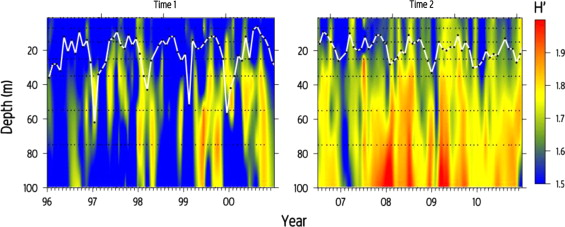
\includegraphics[trim = 0mm 0mm 0mm 0mm, clip, width=.8\linewidth]{./Chp3-Further/PinckneyDiversityPigmentData.jpg}
\caption[Scheme]{\small {"Time series contour plot of photopigment diversity index (H′). Data points are indicated by dots on the plot and the white line shows the mixed layer depth." from \citet{Pinckney2015}}}
\label{PrinComp}
\end{figure}

%this needs proper formatting still man

\begin{figure}
\centering
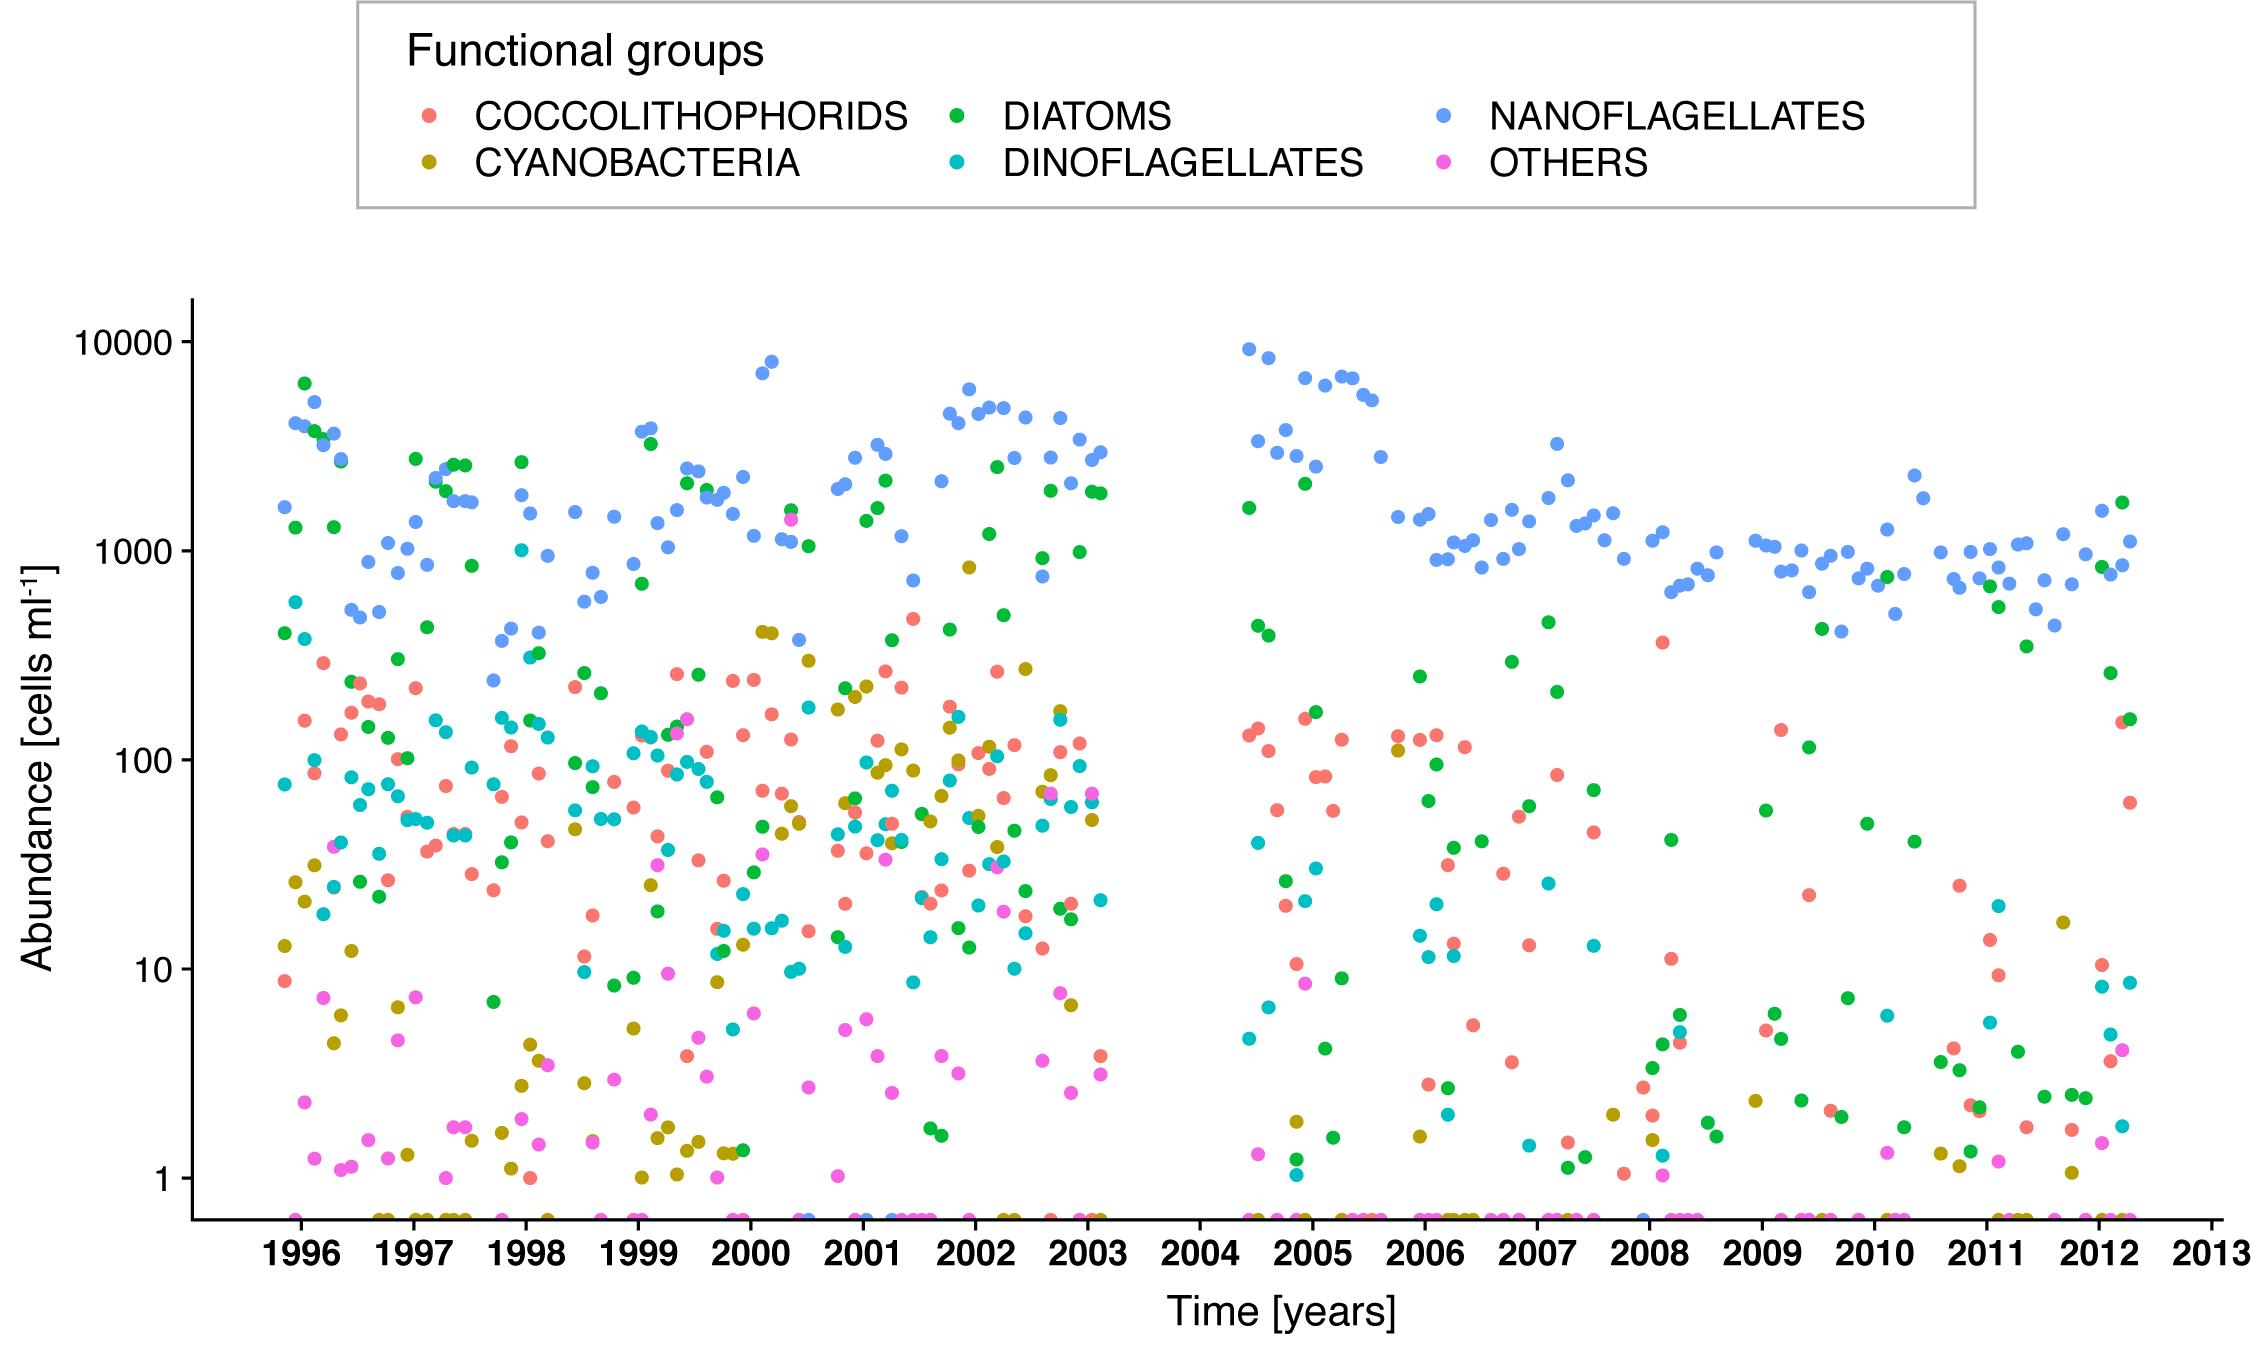
\includegraphics[trim = 0mm 0mm 0mm 0mm, clip, width=1.\linewidth]{./Chp3-Further/AbundancesAsset111.png}
\caption[Scheme]{\small {Abundances per functional group in phytoplankton taxonomy data of CARIACO time-series. Phytoplankton species were identified using light microscopy and identified down to genus or species level.}}
\label{Abundances}
\end{figure}
% need to edit in illustrator



\section{Time Table}

\begin{figure}[h]
\centering
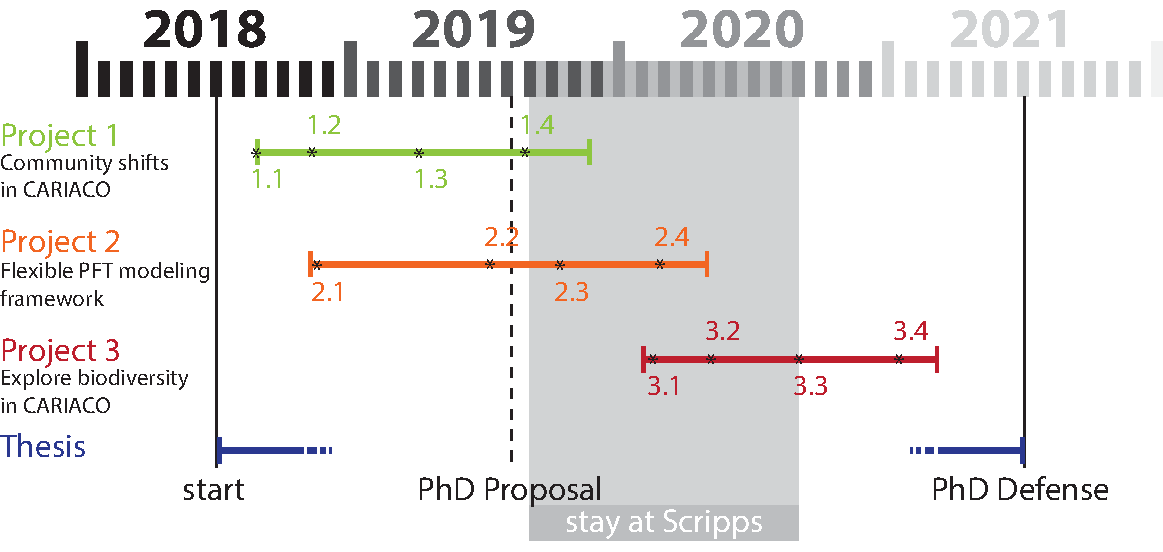
\includegraphics[trim = 0mm 0mm 0mm 0mm, clip, width=1.1\linewidth]{./Chp3-Further/TimePlanAsset1.pdf}

\end{figure}


The first 2 months of the PhD were spent working on a review of the current scientific literature .

{\bf{Project 1 - Understanding community shifts}}

\noindent
1.1: Finding public ocean time-series to use for phytoplankton ecosystem modeling.\\
\noindent
1.2: Analyzing CARIACO time-series data and creating a model construct to test hypotheses.\\
\noindent
1.3: After receiving HPLC data from James Pinckney and Claudia Benitez-Nelson, the model ecosystem structure was finalized. \\
\noindent
1.4: Model physics need to be finalized, to create baseline run with the regime 1 forcing. Then start hypothesis testing, generating final results and writing up the manuscript in the following months. \\


{\bf{Project 2 - PhytoMFTM}}

\noindent
2.1: Idea for flexible object-oriented model was developed, first code testing.\\
\noindent
2.2: Code structure was optimized for usage for Project 1.\\
\noindent
2.3: Upon arriving at Scripps, I will discuss possible model structures for Project 3 with Andrew Barton and modify the model package accordingly. \\
\noindent
2.4: Prepare model code for package deployment and start writing technical manuscript describing code function and structure. \\
% EST: FYI in GMD the interest is not about the code per se so do not put so much emphasis in the code


{\bf{Project 3 - BDEF in Cariaco}}

\noindent
3.1: Settle on hypothesis and model structure together with Andrew Barton, start specific data analysis of CARIACO time-series data relevant to the question.\\
\noindent
3.2: Finish data analysis of diversity related data and start implementing the model with the finished PhytoMFTM framework.\\
\noindent
3.3: Start hypothesis testing and parameter fitting. \\
\noindent
3.4: Finish up results and start writing manuscript. \\


The last 3 months of the PhD are reserved for writing up the thesis and preparing PhD Defense.

